\section{User Study}
We conducted a user study to examine the productivity of our system in constructing the corresponding 3D model of the planar layout, and the guiding effectiveness of users fabricating the practical mockup. The experiment was separated into two parts. In the first experiment, participants were asked to construct the 3D model from the same 2D layout using our system and STUDIO after a brief introduction, and a two-alternative forced choices design was used, with participants asked to choose which system they preferred to use considering the complexity of operations or modeling time. Furthermore, participants needed to rate our system from one to five on the necessity of layout optimization, five is for very necessary. In the second experiment, participants were separated equally into two groups, one group was asked to fold the given practical printed paper into 3D mockup with the guide video showing the folding sequence provided by our system and the fabrication time was recorded compared with another group without the guide video. Our goal was to test the following hypotheses:

\begin{itemize}
	\item \textbf{Hypo1:} Our system need less time and effort to construct a digital 3D mockup than traditional software.
	\item \textbf{Hypo2:} Our system can provide novel and practical function to reach diverse layouts.
	\item \textbf{Hypo3:} Our system can guide the fabrication of cartons.
\end{itemize}

\subsection{Procedure}
We began the experiment with each participant by explaining the background and the instructions of our system and STUDIO. Ten layouts from thirty-four 2D design layouts were given to participants for folding, and at least three of them would need refinement. Participants were allowed to watch the final model of the layout to instruct construction. After operating the two systems. each participant was asked to answer a questionnaire including four(??five?? not clear how to use the question of modeling experiment) questions: which of two systems participants preferred based on the simplicity of operation. which of two systems participants preferred based on the modeling time, score one to five on the necessity of layout optimization in our system. and write down the suggestions to our system.

Foe the second experiment, we separated participants into two groups, one group would fabricate the layout as shown in Figure~\ref{fig:automatic-more}(a) with a video presenting the folding sequence, and another group would fold the layout with a figure showing the layout and its final model instead of video. The fabrication time was recorded for analysis. 

\subsection{Discussion}
We consider our three hypotheses in turn. With respect to Hypo1, we collect the answers of former two questions from 30 participants, the result is show in Figure~\ref{fig:preference}. We also performed a pared-samples t-test at level $\alpha = 0.05$ to compare the preference significance, and the test shows our system is significant preferred by participants.(?How to show t-test result?) Considering the suggestions from participants preferring STUDIO, the operations need to be learned from STUDIO is just selecting folding lines and assigning angles, while ours provides multiple selections to construct the final model. However, when most participants think the steps need to take to final model is much less than STUDIO, which is the main reason choosing our system. Take Figure~\ref{fig:result-more}(e) for example, participants usually took much time to slightly adjust the folding angles of creases, while ours just needs three clicks.


\begin{figure}
	\centering
	\subfigure[Preference System]{
		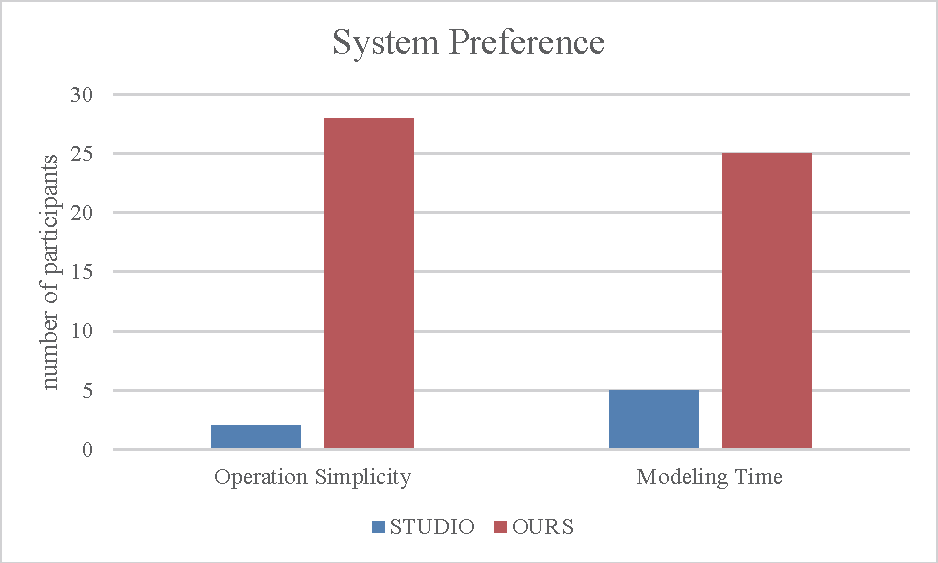
\includegraphics[width=0.45\columnwidth,height=0.17\textheight]{images/preference.png}
		\label{fig:preference}
	}
	\vspace{-1ex}
	\subfigure[Fabrication Time]{
		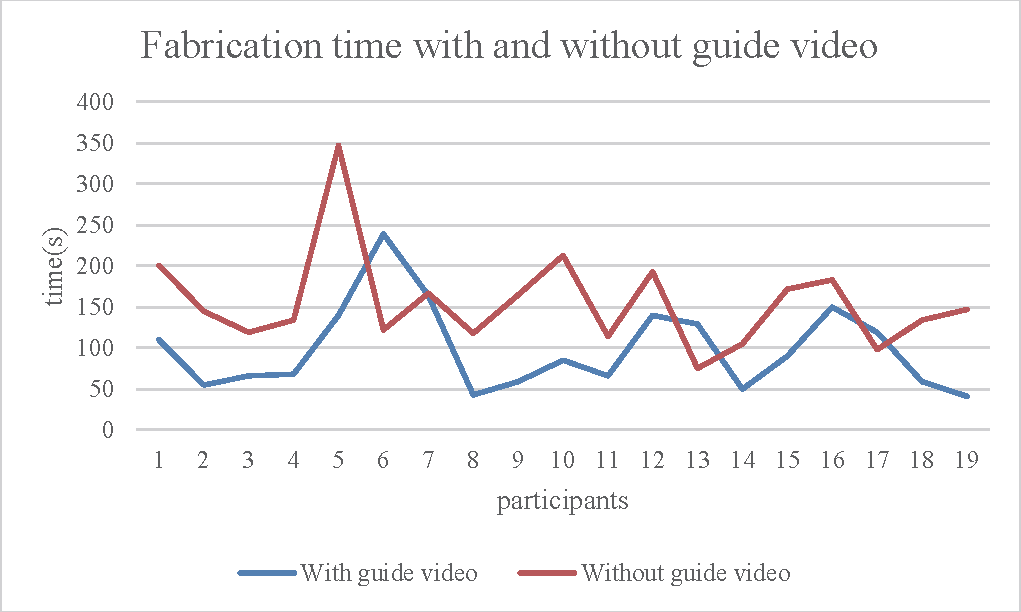
\includegraphics[width=0.45\columnwidth,height=0.17\textheight]{images/fabrication.png}
		\label{fig:time}
	}
	\caption{(a) shows the collection of the former two answers related to the preference based on modeling time and operation simplicity. (b) shows the fabrication time with or without video.  }
	\label{fig:data}
\end{figure}

With respect to Hypo2, twenty-four participants gave the highest score to our layout optimization function. In addition to explore the diversity of 2D layouts, it also can adjust the imprecise faces on 2D layout to reach an ideal model by construction. Figure~\ref{fig:correction} shows the final model constructed by our system and STUDIO, as we can see, the side face 1 is higher than face 2 in the model constructed by STUDIO, while in our system, we can correct these design error by merging vertices circled in red.

\begin{figure}
	\centering
	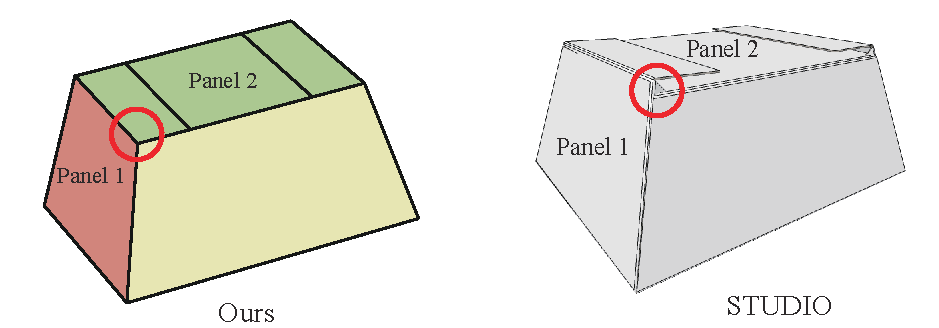
\includegraphics[width=0.5\textwidth]{images/comparison}
	\caption{Different model constructed by our system (a) and STUDIO (b). }
	\label{fig:correction}
\end{figure}

For Hypo3, 38 participants were asked to fabricate the practical layout into corresponding model, and the fabrication time is shown in Figure~\ref{fig:time}. As we can see, most participants which have not seen the guide video took more time to fold the carton than another group. We also performed an independent-samples t test at level $\alpha = 0.05$ to compare the fabrication time, and the result shows the guide video has significant effectiveness on the fabrication of complex cartons.




